%% Преамбула TeX-файла

% 1. Стиль и язык
\documentclass[utf8x, 12pt]{G7-32} % Стиль (по умолчанию будет 14pt)

% Остальные стандартные настройки убраны в preamble.inc.tex.
\sloppy

% Настройки стиля ГОСТ 7-32
% Для начала определяем, хотим мы или нет, чтобы рисунки и таблицы нумеровались в пределах раздела, или нам нужна сквозная нумерация.
\EqInChapter % формулы будут нумероваться в пределах раздела
\TableInChapter % таблицы будут нумероваться в пределах раздела
\PicInChapter % рисунки будут нумероваться в пределах раздела
\usepackage{slashbox}

% Добавляем гипертекстовое оглавление в PDF
\usepackage[
bookmarks=true, colorlinks=true, unicode=true,
urlcolor=black,linkcolor=black, anchorcolor=black,
citecolor=black, menucolor=black, filecolor=black,
]{hyperref}

% Изменение начертания шрифта --- после чего выглядит таймсоподобно.
% apt-get install scalable-cyrfonts-tex

\IfFileExists{cyrtimes.sty}
    {
        \usepackage{cyrtimespatched}
    }
    {
        % А если Times нету, то будет CM...
    }

\usepackage{graphicx}   % Пакет для включения рисунков

% С такими оно полями оно работает по-умолчанию:
% \RequirePackage[left=20mm,right=10mm,top=20mm,bottom=20mm,headsep=0pt]{geometry}
% Если вас тошнит от поля в 10мм --- увеличивайте до 20-ти, ну и про переплёт не забывайте:
\geometry{right=20mm}
\geometry{left=30mm}


% Пакет Tikz
\usepackage{tikz}
\usetikzlibrary{arrows,positioning,shadows}

% Произвольная нумерация списков.
\usepackage{enumerate}

% ячейки в несколько строчек
\usepackage{multirow}

% itemize внутри tabular
\usepackage{paralist,array}

% Центрирование подписей к плавающим окружениям
\usepackage[justification=centering]{caption}


% Настройки листингов.
\ifPDFTeX
% 8 Листинги

\usepackage{listings}
\usepackage{wrapfig}
% Значения по умолчанию
\lstset{
  basicstyle= \footnotesize,
  breakatwhitespace=true,% разрыв строк только на whitespacce
  breaklines=true,       % переносить длинные строки
%   captionpos=b,          % подписи снизу -- вроде не надо
  inputencoding=koi8-r,
  numbers=left,          % нумерация слева
  numberstyle=\footnotesize,
  showspaces=false,      % показывать пробелы подчеркиваниями -- идиотизм 70-х годов
  showstringspaces=false,
  showtabs=false,        % и табы тоже
  stepnumber=1,
  tabsize=4,              % кому нужны табы по 8 символов?
  frame=single
}

% Стиль для псевдокода: строчки обычно короткие, поэтому размер шрифта побольше
\lstdefinestyle{pseudocode}{
  basicstyle=\small,
  keywordstyle=\color{black}\bfseries\underbar,
  language=Pseudocode,
  numberstyle=\footnotesize,
  commentstyle=\footnotesize\it
}

% Стиль для обычного кода: маленький шрифт
\lstdefinestyle{realcode}{
  basicstyle=\scriptsize,
  numberstyle=\footnotesize
}

% Стиль для коротких кусков обычного кода: средний шрифт
\lstdefinestyle{simplecode}{
  basicstyle=\footnotesize,
  numberstyle=\footnotesize
}

% Стиль для BNF
\lstdefinestyle{grammar}{
  basicstyle=\footnotesize,
  numberstyle=\footnotesize,
  stringstyle=\bfseries\ttfamily,
  language=BNF
}

% Определим свой язык для написания псевдокодов на основе Python
\lstdefinelanguage[]{Pseudocode}[]{Python}{
  morekeywords={each,empty,wait,do},% ключевые слова добавлять сюда
  morecomment=[s]{\{}{\}},% комменты {а-ля Pascal} смотрятся нагляднее
  literate=% а сюда добавлять операторы, которые хотите отображать как мат. символы
    {->}{\ensuremath{$\rightarrow$}~}2%
    {<-}{\ensuremath{$\leftarrow$}~}2%
    {:=}{\ensuremath{$\leftarrow$}~}2%
    {<--}{\ensuremath{$\Longleftarrow$}~}2%
}[keywords,comments]

% Свой язык для задания грамматик в BNF
\lstdefinelanguage[]{BNF}[]{}{
  morekeywords={},
  morecomment=[s]{@}{@},
  morestring=[b]",%
  literate=%
    {->}{\ensuremath{$\rightarrow$}~}2%
    {*}{\ensuremath{$^*$}~}2%
    {+}{\ensuremath{$^+$}~}2%
    {|}{\ensuremath{$|$}~}2%
}[keywords,comments,strings]

% Подписи к листингам на русском языке.
\renewcommand\lstlistingname{\cyr\CYRL\cyri\cyrs\cyrt\cyri\cyrn\cyrg}
\renewcommand\lstlistlistingname{\cyr\CYRL\cyri\cyrs\cyrt\cyri\cyrn\cyrg\cyri}

\else
\usepackage{local-minted}
\fi
\usepackage{dirtytalk}
\usepackage{algorithm2e}
\usepackage[noend]{algpseudocode}
\usepackage{csquotes}
\usepackage[at]{easylist}
\usepackage{pgfplots}

% Полезные макросы листингов.
% Любимые команды
\newcommand{\Code}[1]{\textbf{#1}}


\begin{document}

\frontmatter % выключает нумерацию ВСЕГО; здесь начинаются ненумерованные главы: реферат, введение, глоссарий, сокращения и прочее.

% Команды \breakingbeforechapters и \nonbreakingbeforechapters
% управляют разрывом страницы перед главами.
% По-умолчанию страница разрывается.

% \nobreakingbeforechapters
% \breakingbeforechapters

% НАЧАЛО ТИТУЛЬНОГО ЛИСТА
\begin{center}
	\hfill \break
	\textit{
		\normalsize{Государственное образовательное учреждение высшего профессионального образования}}\\ 
	
	\textit{
		\normalsize  {\bf  «Московский государственный технический университет}\\ 
		\normalsize  {\bf имени Н. Э. Баумана»}\\
		\normalsize  {\bf (МГТУ им. Н.Э. Баумана)}\\
	}
	\noindent\rule{\textwidth}{2pt}
	\hfill \break
	\noindent
	\\
	\noindent
	\\
	\hfill\break
	\hfill \break
	\hfill \break
	\hfill \break
	
	\hfill \break
	\large{Лабораторная работа №2, 4\\ \textquote{Умножение матриц}}\\
	\hfill \break
	\hfill \break
	\hfill \break
	\hfill \break
	\hfill \break	
	\normalsize {
		\begin{minipage}[t]{7cm}
		\end{minipage}
		\hfill
		\begin{minipage}[t]{7cm}
			\flushright
			Студент: Камакин А.С.\\
			Группа: ИУ7-53\\
			Преподаватель: Волкова Л.Л.
		\end{minipage}
	}\\
	\hfill \break	
	\hfill \break
	\hfill \break
	\hfill \break
	\hfill \break
\end{center}
\hfill \break
\hfill \break
\begin{center} Москва 2017 \end{center}

\thispagestyle{empty} % 
% КОНЕЦ ТИТУЛЬНОГО ЛИСТА

\newpage
% \tableofcontents

\mainmatter % это включает нумерацию глав и секций в документе ниже

\paragraph{Системные характеристики и окружение}
\begin{itemize}
	\item Операционная система: Ubuntu 17.10 64-bit
	\item Память: 15,4 GiB
	\item Процессор: Intel® Core™ i5-3320M CPU @ 2.60GHz × 4
\end{itemize}

Пояснение: Стандартная системная утилита показывает, что в системе 4 ядра, но не говорит какие именно. Чтобы точно узнать количество ядер необходимо выполнить одну и следующих команд: cat /proc/cpuinfo | grep 'core id' или lscpu (поле Core(s) per socket)
\\

Пример выполнения команды cat /proc/cpuinfo | grep 'core id':\\
core id		: 0\\
core id		: 0\\
core id		: 1\\
core id		: 1\\

Пример выполнения команды lscpu:\\
CPU op-mode(s):      32-bit, 64-bit\\
Byte Order:          Little Endian\\
CPU(s):              4\\
On-line CPU(s) list: 0-3\\
Thread(s) per core:  2\\
Core(s) per socket:  2\\
Socket(s):           1\\
NUMA node(s):        1\\
Vendor ID:           GenuineIntel\\
CPU family:          6\\
Model:               58\\
Model name:          Intel(R) Core(TM) i5-3320M CPU @ 2.60GHz\\
Stepping:            9\\
CPU MHz:             2594.117\\
CPU max MHz:         3300,0000\\
CPU min MHz:         1200,0000\\
BogoMIPS:            5188.23\\
Virtualization:      VT-x\\

Можно сделать вывод, что у тестируемой среды есть 2 реальных и 4 логических ядра, что достигается за счет технологии hyperthreading.

\newpage

\paragraph{Терминология}
\\
Бенчмарк - эталонный тест производительности компьютерной системы.\\
gobench - инструмент для проведения бенчмарков в языке Go.\\
Горутина (goroutine) - легковесный поток.\\
\\
Отличия горутины от потока:

\begin{itemize}
	\item Можно запустить больше горутин на ОС чем потоков
	\item У горутин динамически растущий по мере необходимости сегментный стек
	\item Время старта горутины меньше чем у потока
	\item Горутины поставляются с механизмом безопасного общения - каналами
	\item Горутины позволяют избежать мьютекса для предоставления доступа к ресурсам
	\item Горутины мультиплексируются на небольшое количество потоков ОС, а не на отображение 1:1.
\end{itemize}

\newpage

Введём модель вычисления, используемую при оценках трудоёмкости:
\begin{itemize}
	\item вызов метода объекта структуры имеет трудоёмкость 1;
	\item объявление переменной/массива/структуры без определения имеет трудоёмкость 0;
	\item операторы $+$, $-$, $*$, $/$, $=$, $++$, $--$ имеют трудоёмкость 1;
	\item условный оператор (без условий внутри) имеет трудоёмкость 0;
	\item логические операции имеют трудоёмкость 1; 
	\item оператор цикла имеет трудоёмкость $1 + n(3 + T)$, где $n$ – это число повторений цикла, $T$ – трудоёмкость тела цикла;
	\begin{itemize}
		\item \textbf{Замечание:} так как доподлинно неизвестно, каким образом компилятор интерпретирует цикл, целесообразно взять модель, предложенную на преподавателем: одно присваивание до цикла (1 операция), внутри цикла присваивание, сравнение и инкремент (3 операции).
	\end{itemize}
	\item вызов функции имеет трудоёмкость 0, так как функции компилятор рассматривает как inline и подставляет сразу вместо вызова код.
	\item $Fn(n)$ – часть трудоёмкости, зависящая только от размера входа;
	\item $g(D)$ – часть трудоёмкости, зависящая от конкретного входа, значений переменных.
\end{itemize}

\newpage

\paragraph{Классический алгоритм перемножения матриц}
\begin{center}
	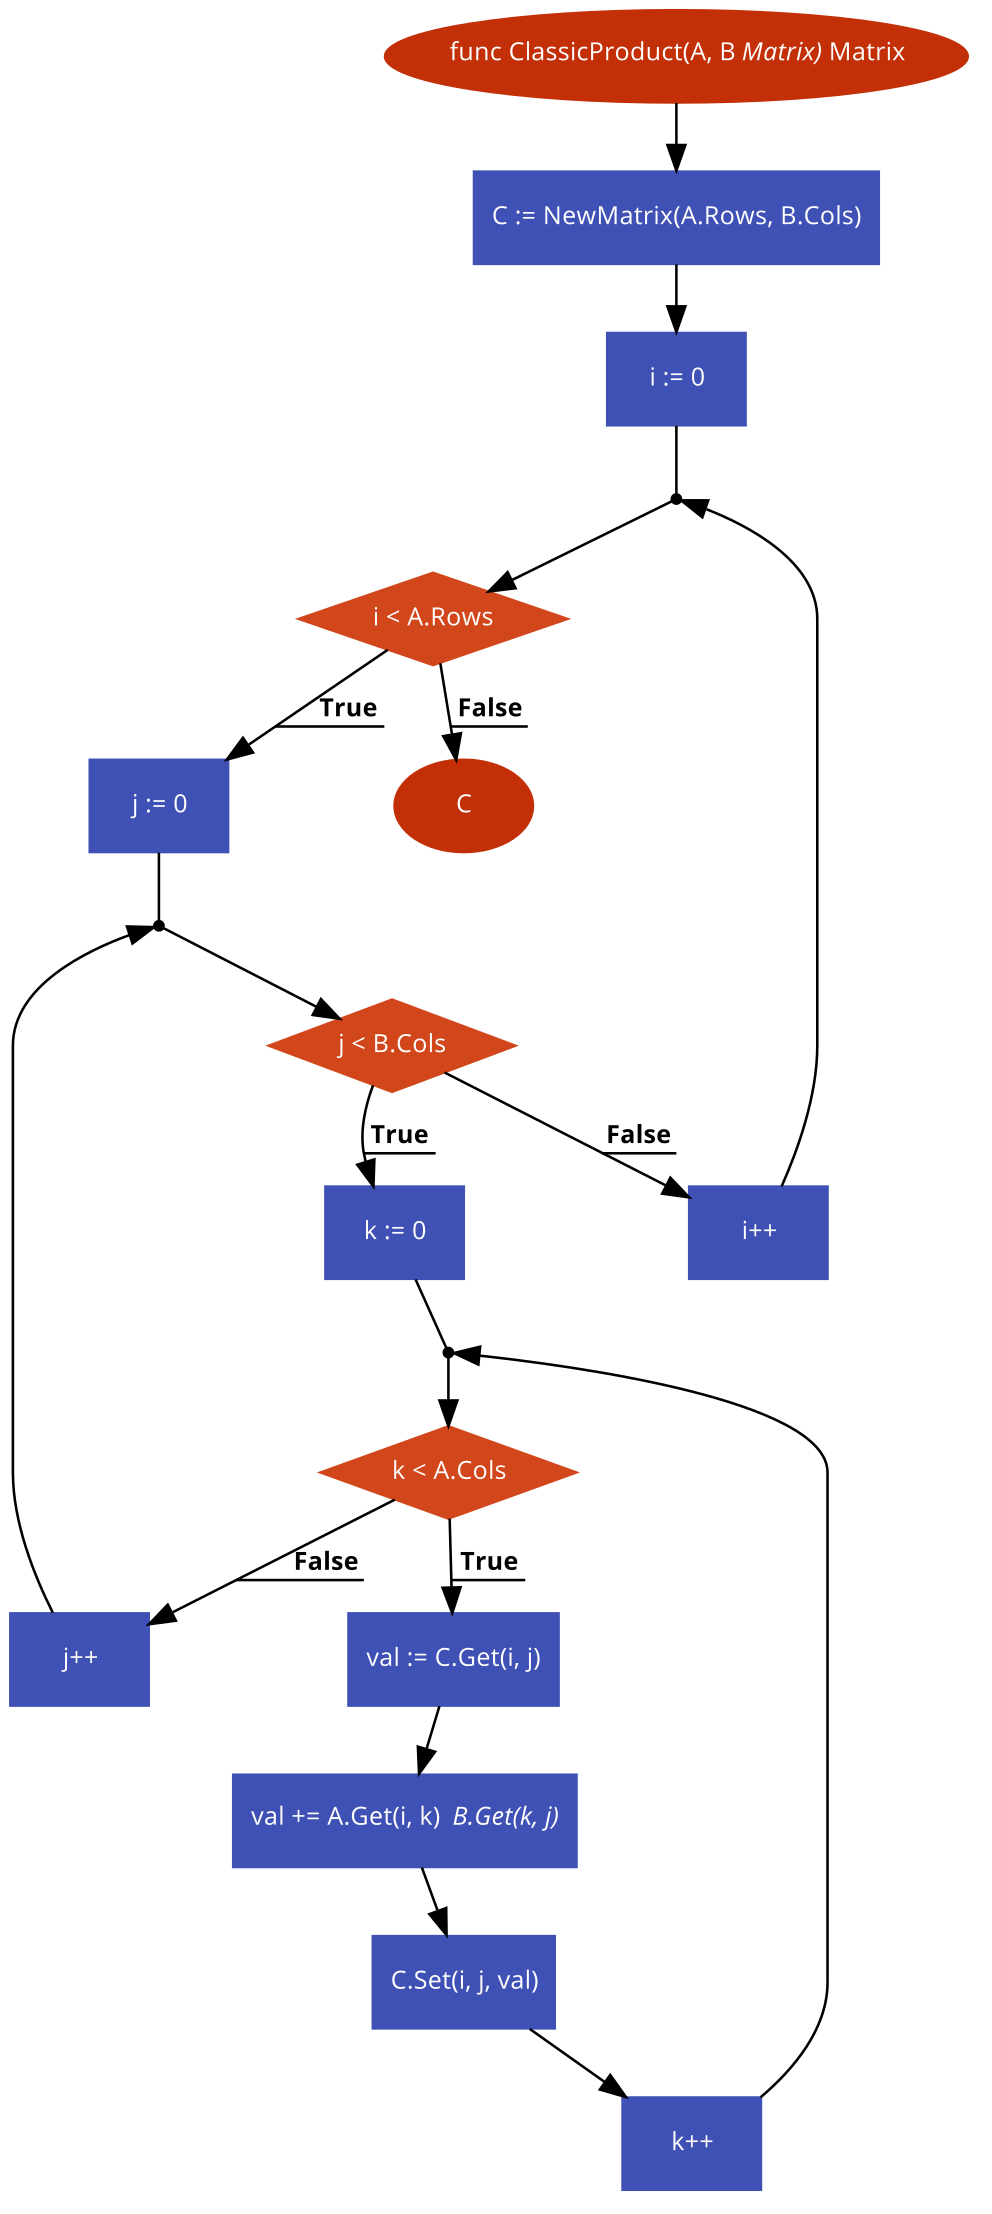
\includegraphics[scale=0.32]{images/matrixClassic.png}
\end{center}

\newpage

\paragraph{Классический алгоритм перемножения матриц с буффером}
\begin{center}
	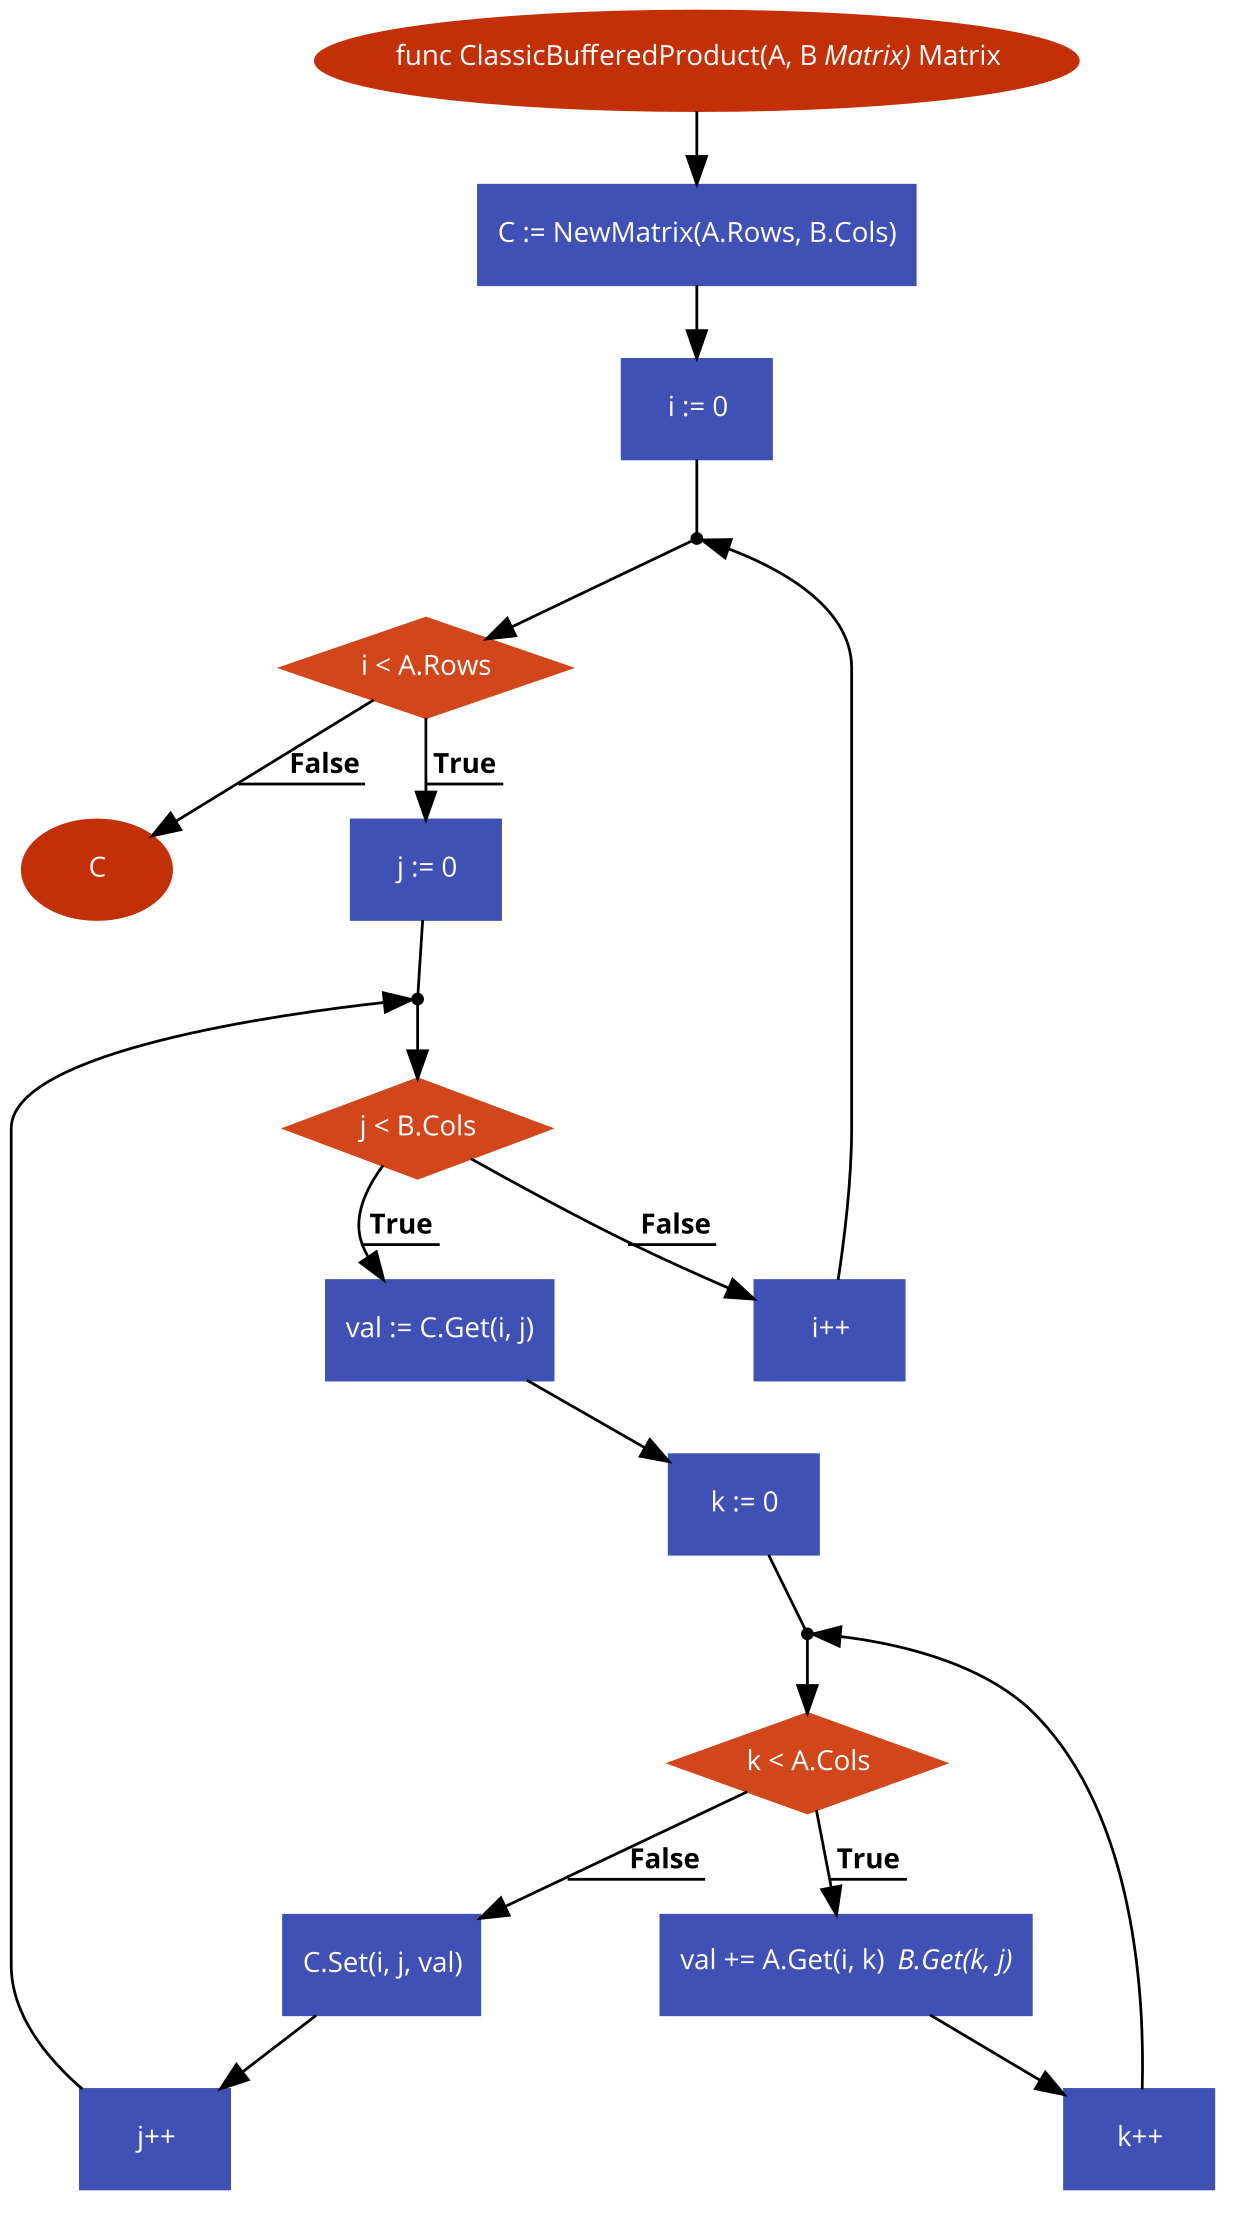
\includegraphics[scale=0.32]{images/matrixClassicBuffered.png}
\end{center}

\newpage

\paragraph{Алгорим Винограда перемножения матриц}
\begin{center}
	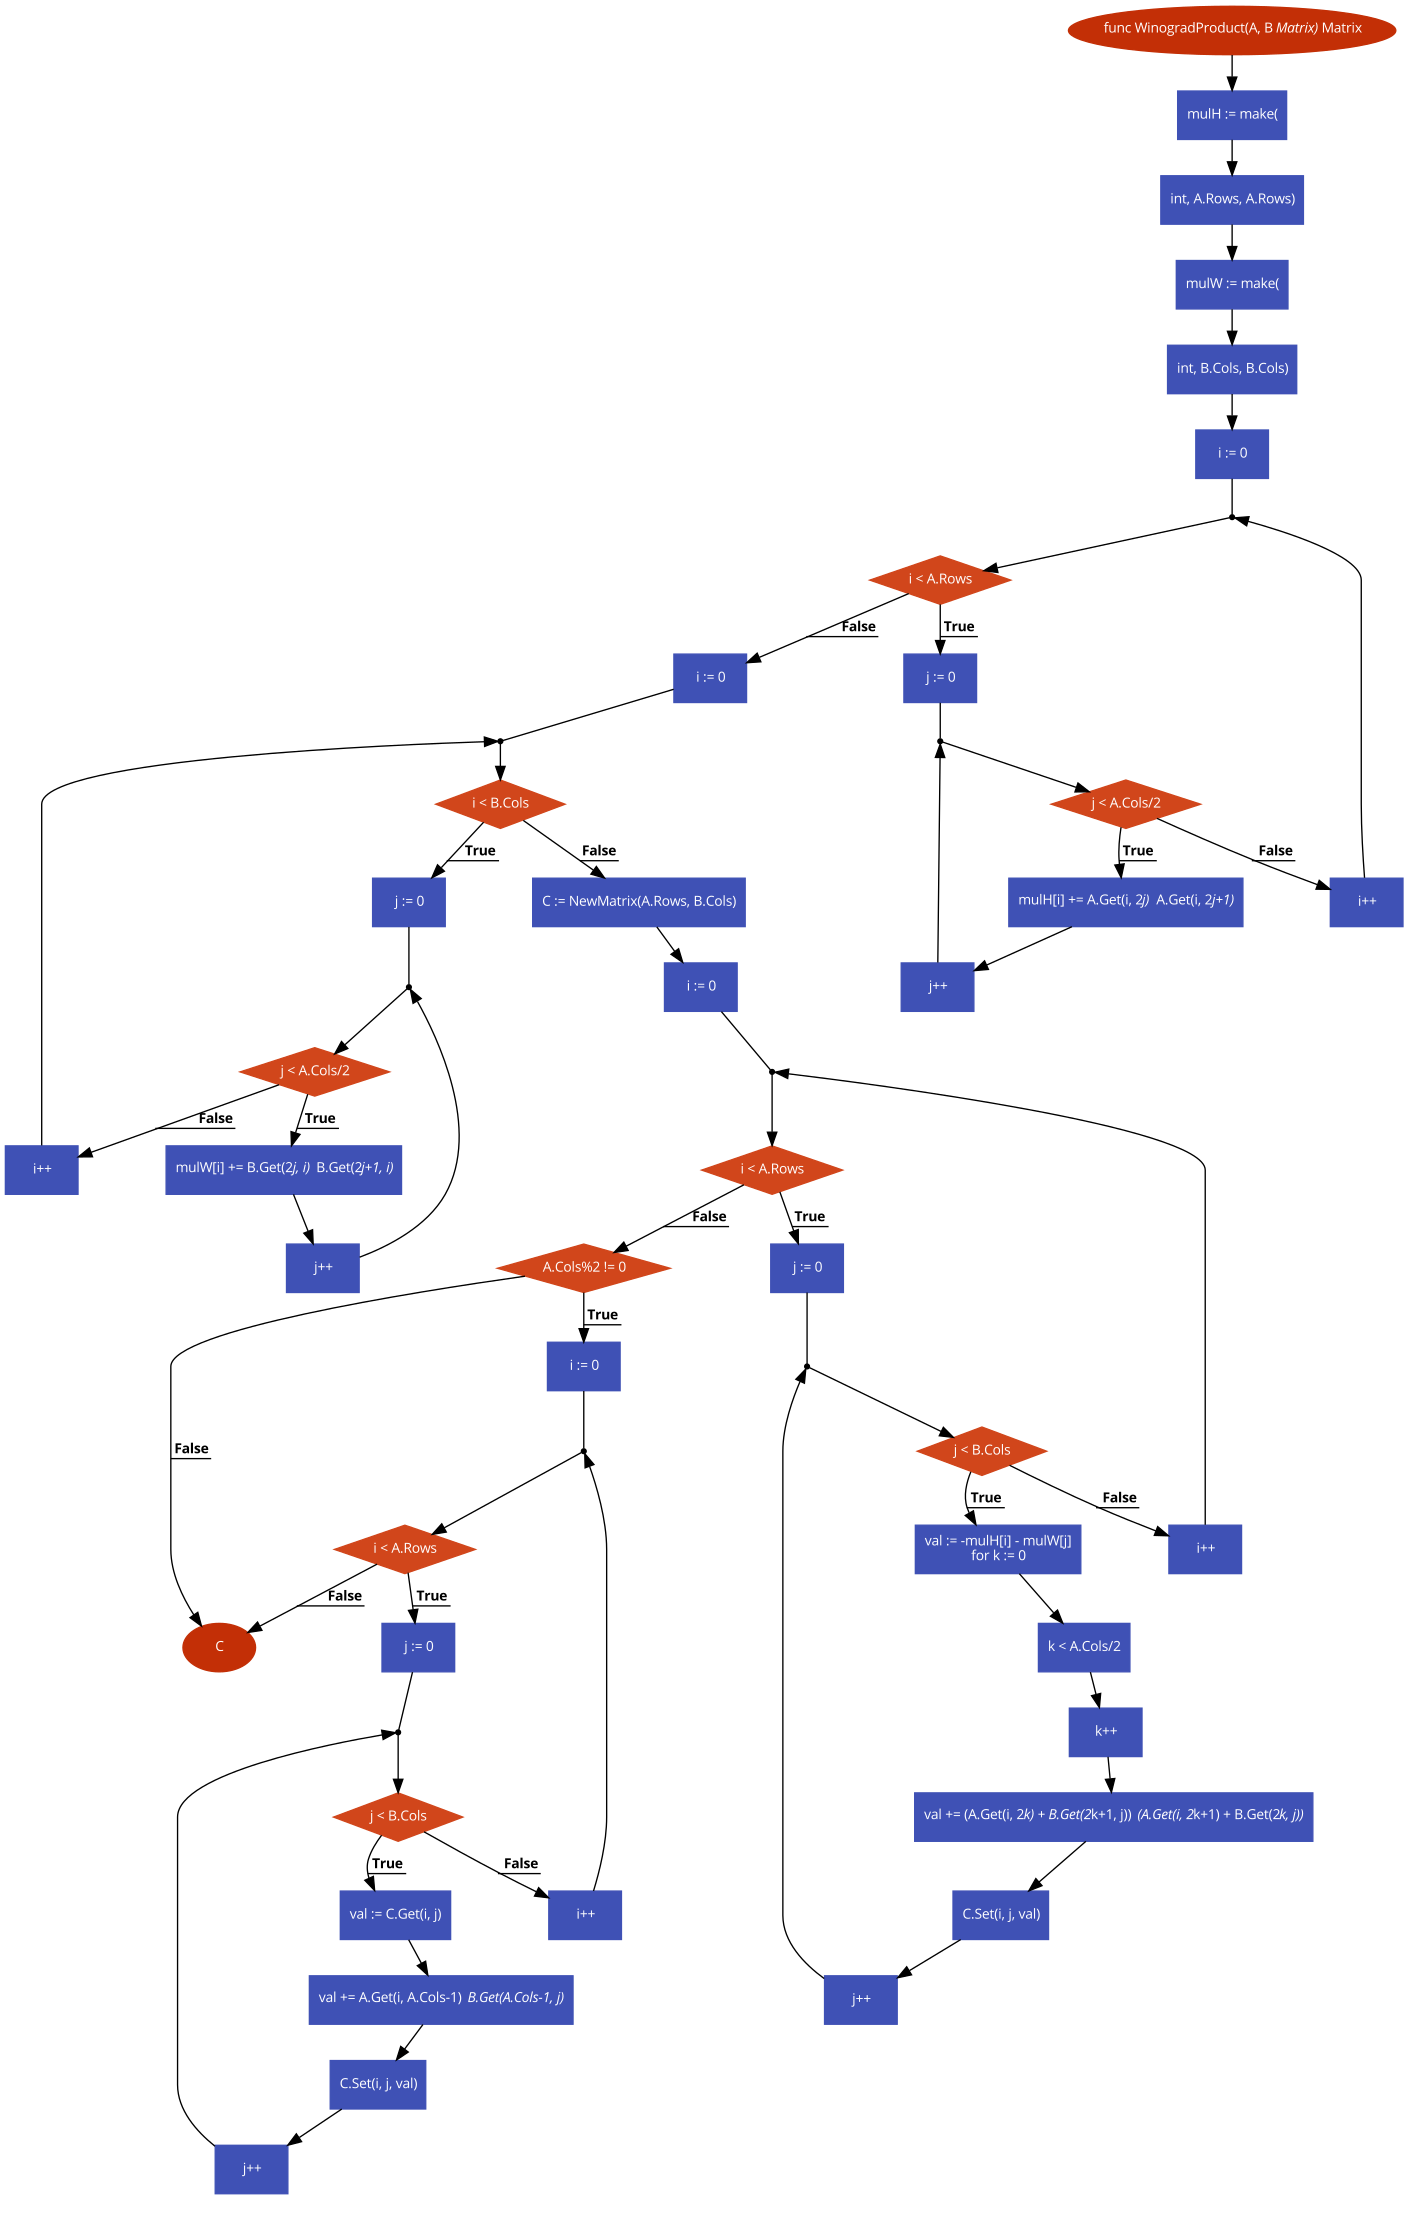
\includegraphics[scale=0.3]{images/matrixWinograd.png}
\end{center}

\newpage

\paragraph{Алгорим Винограда перемножения матриц модифицированный}
\begin{center}
	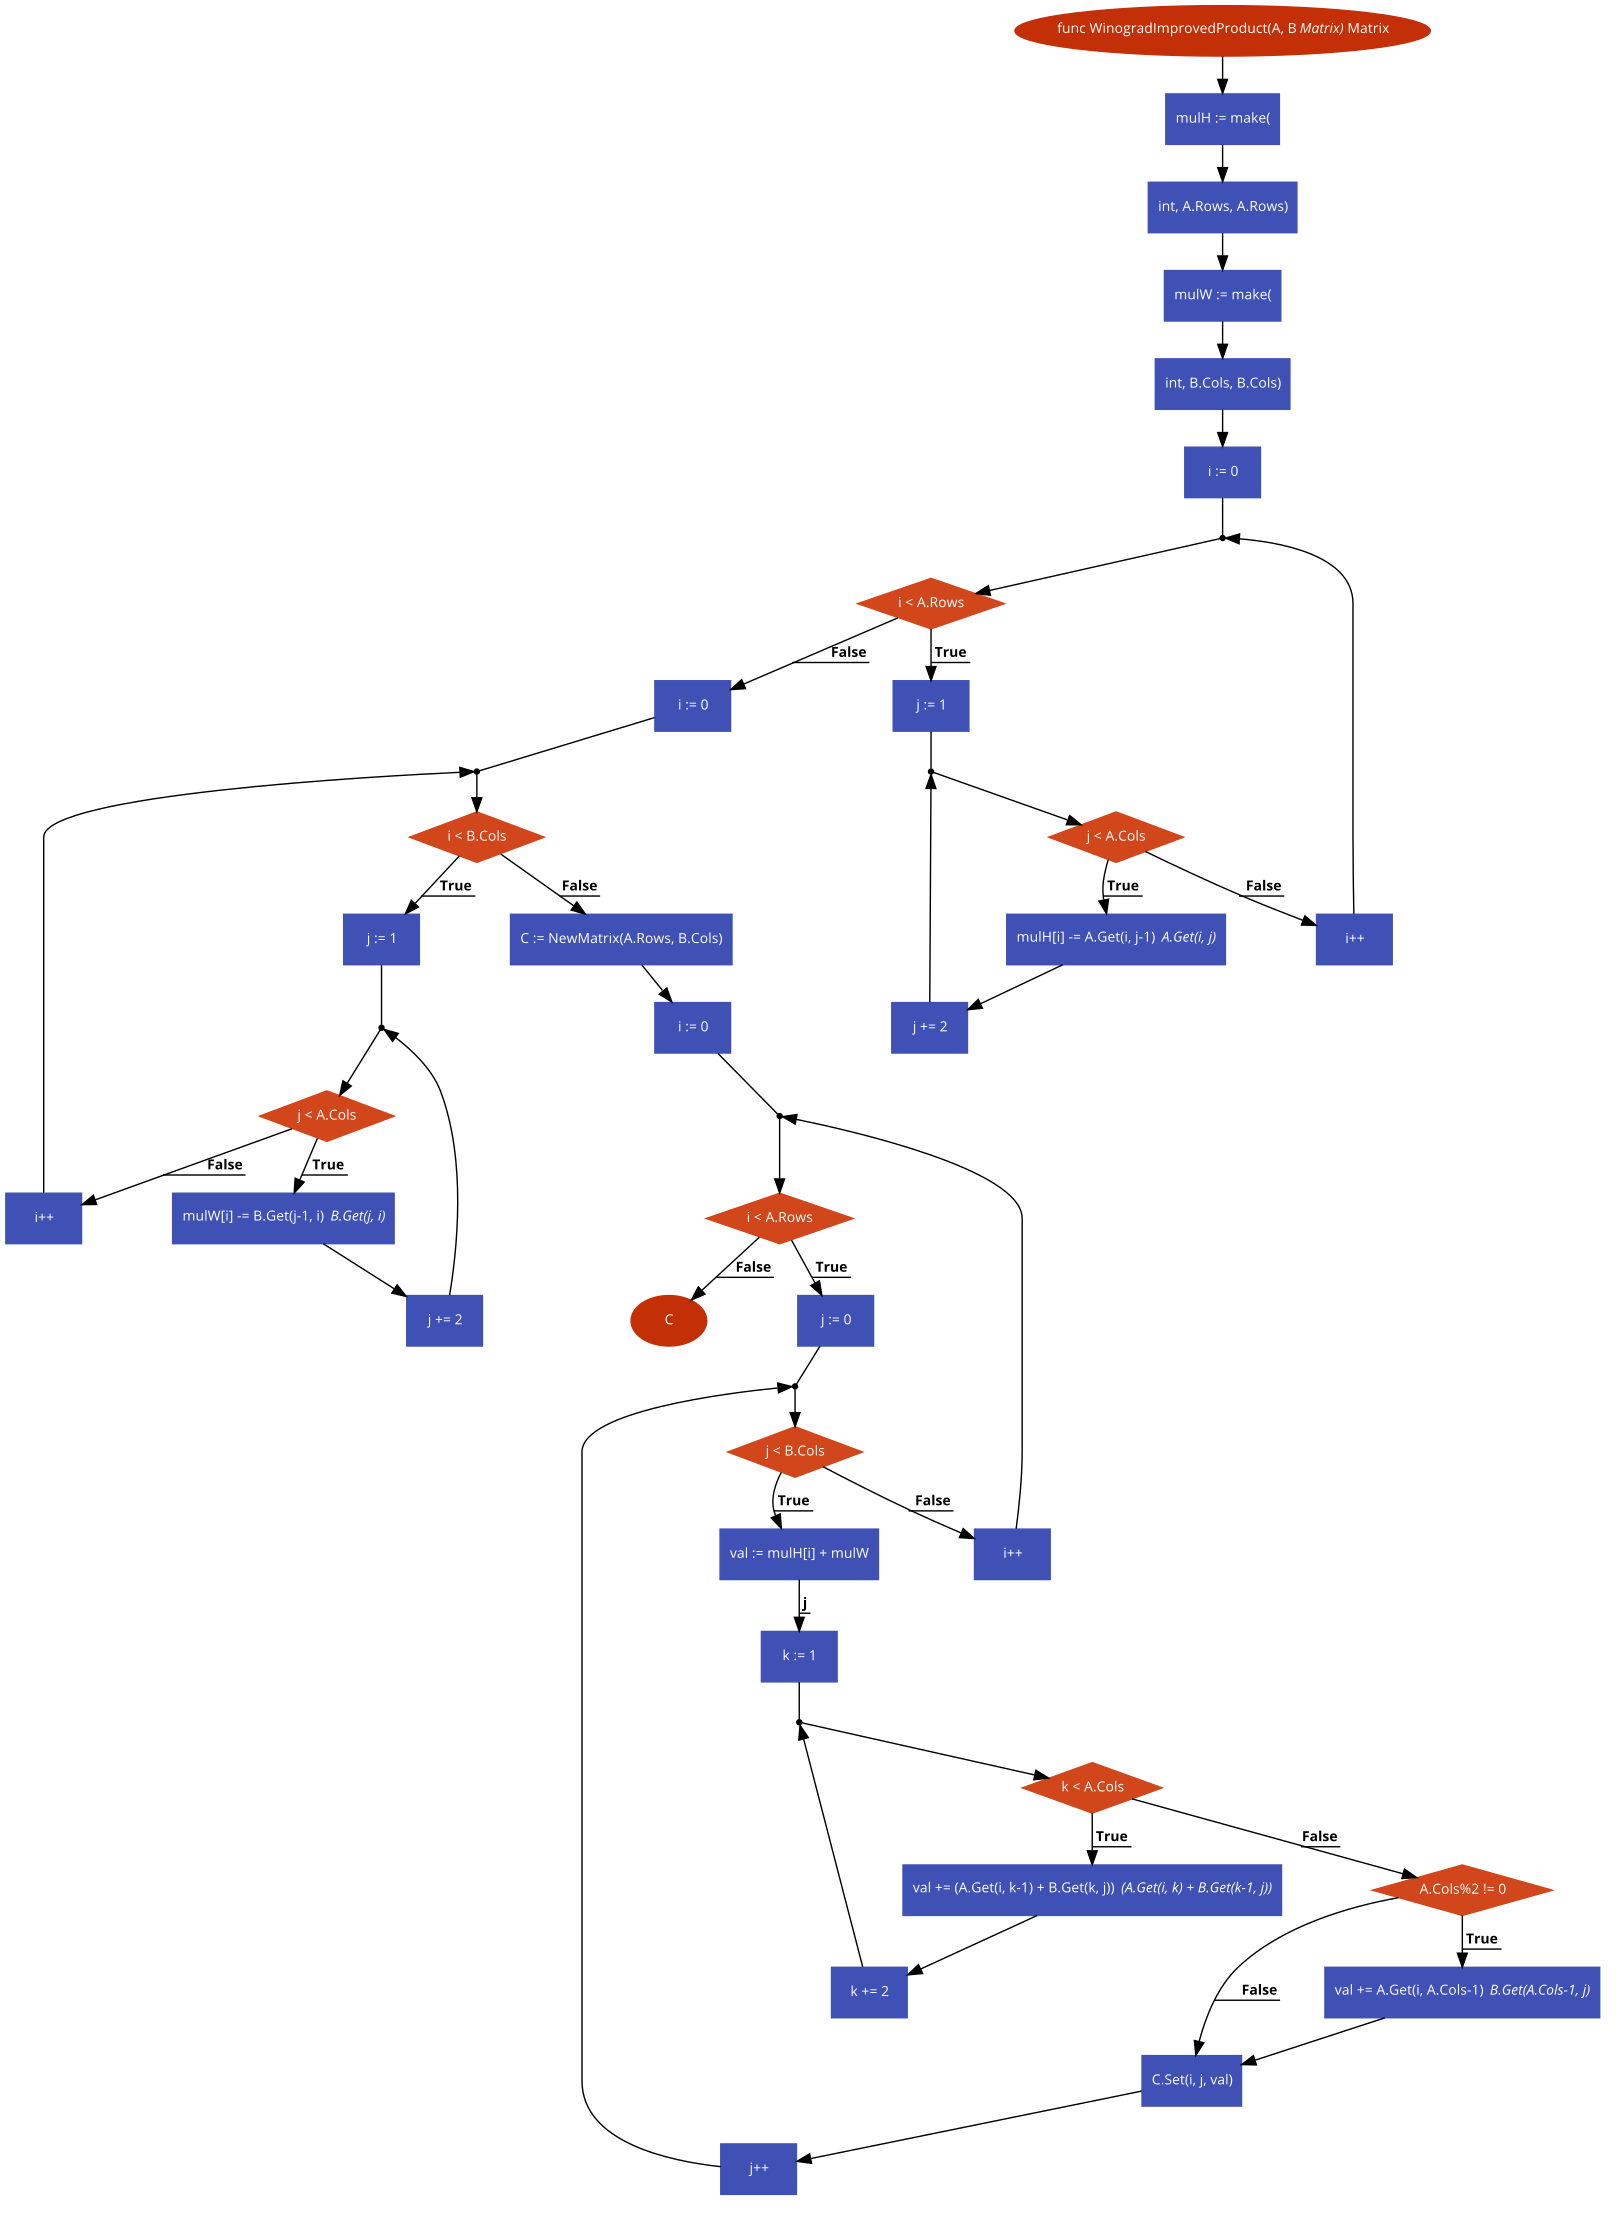
\includegraphics[scale=0.3]{images/matrixWinogradImproved.png}
\end{center}

\newpage

\paragraph{Параллельный алгоритм перемножения матриц}
\begin{center}
	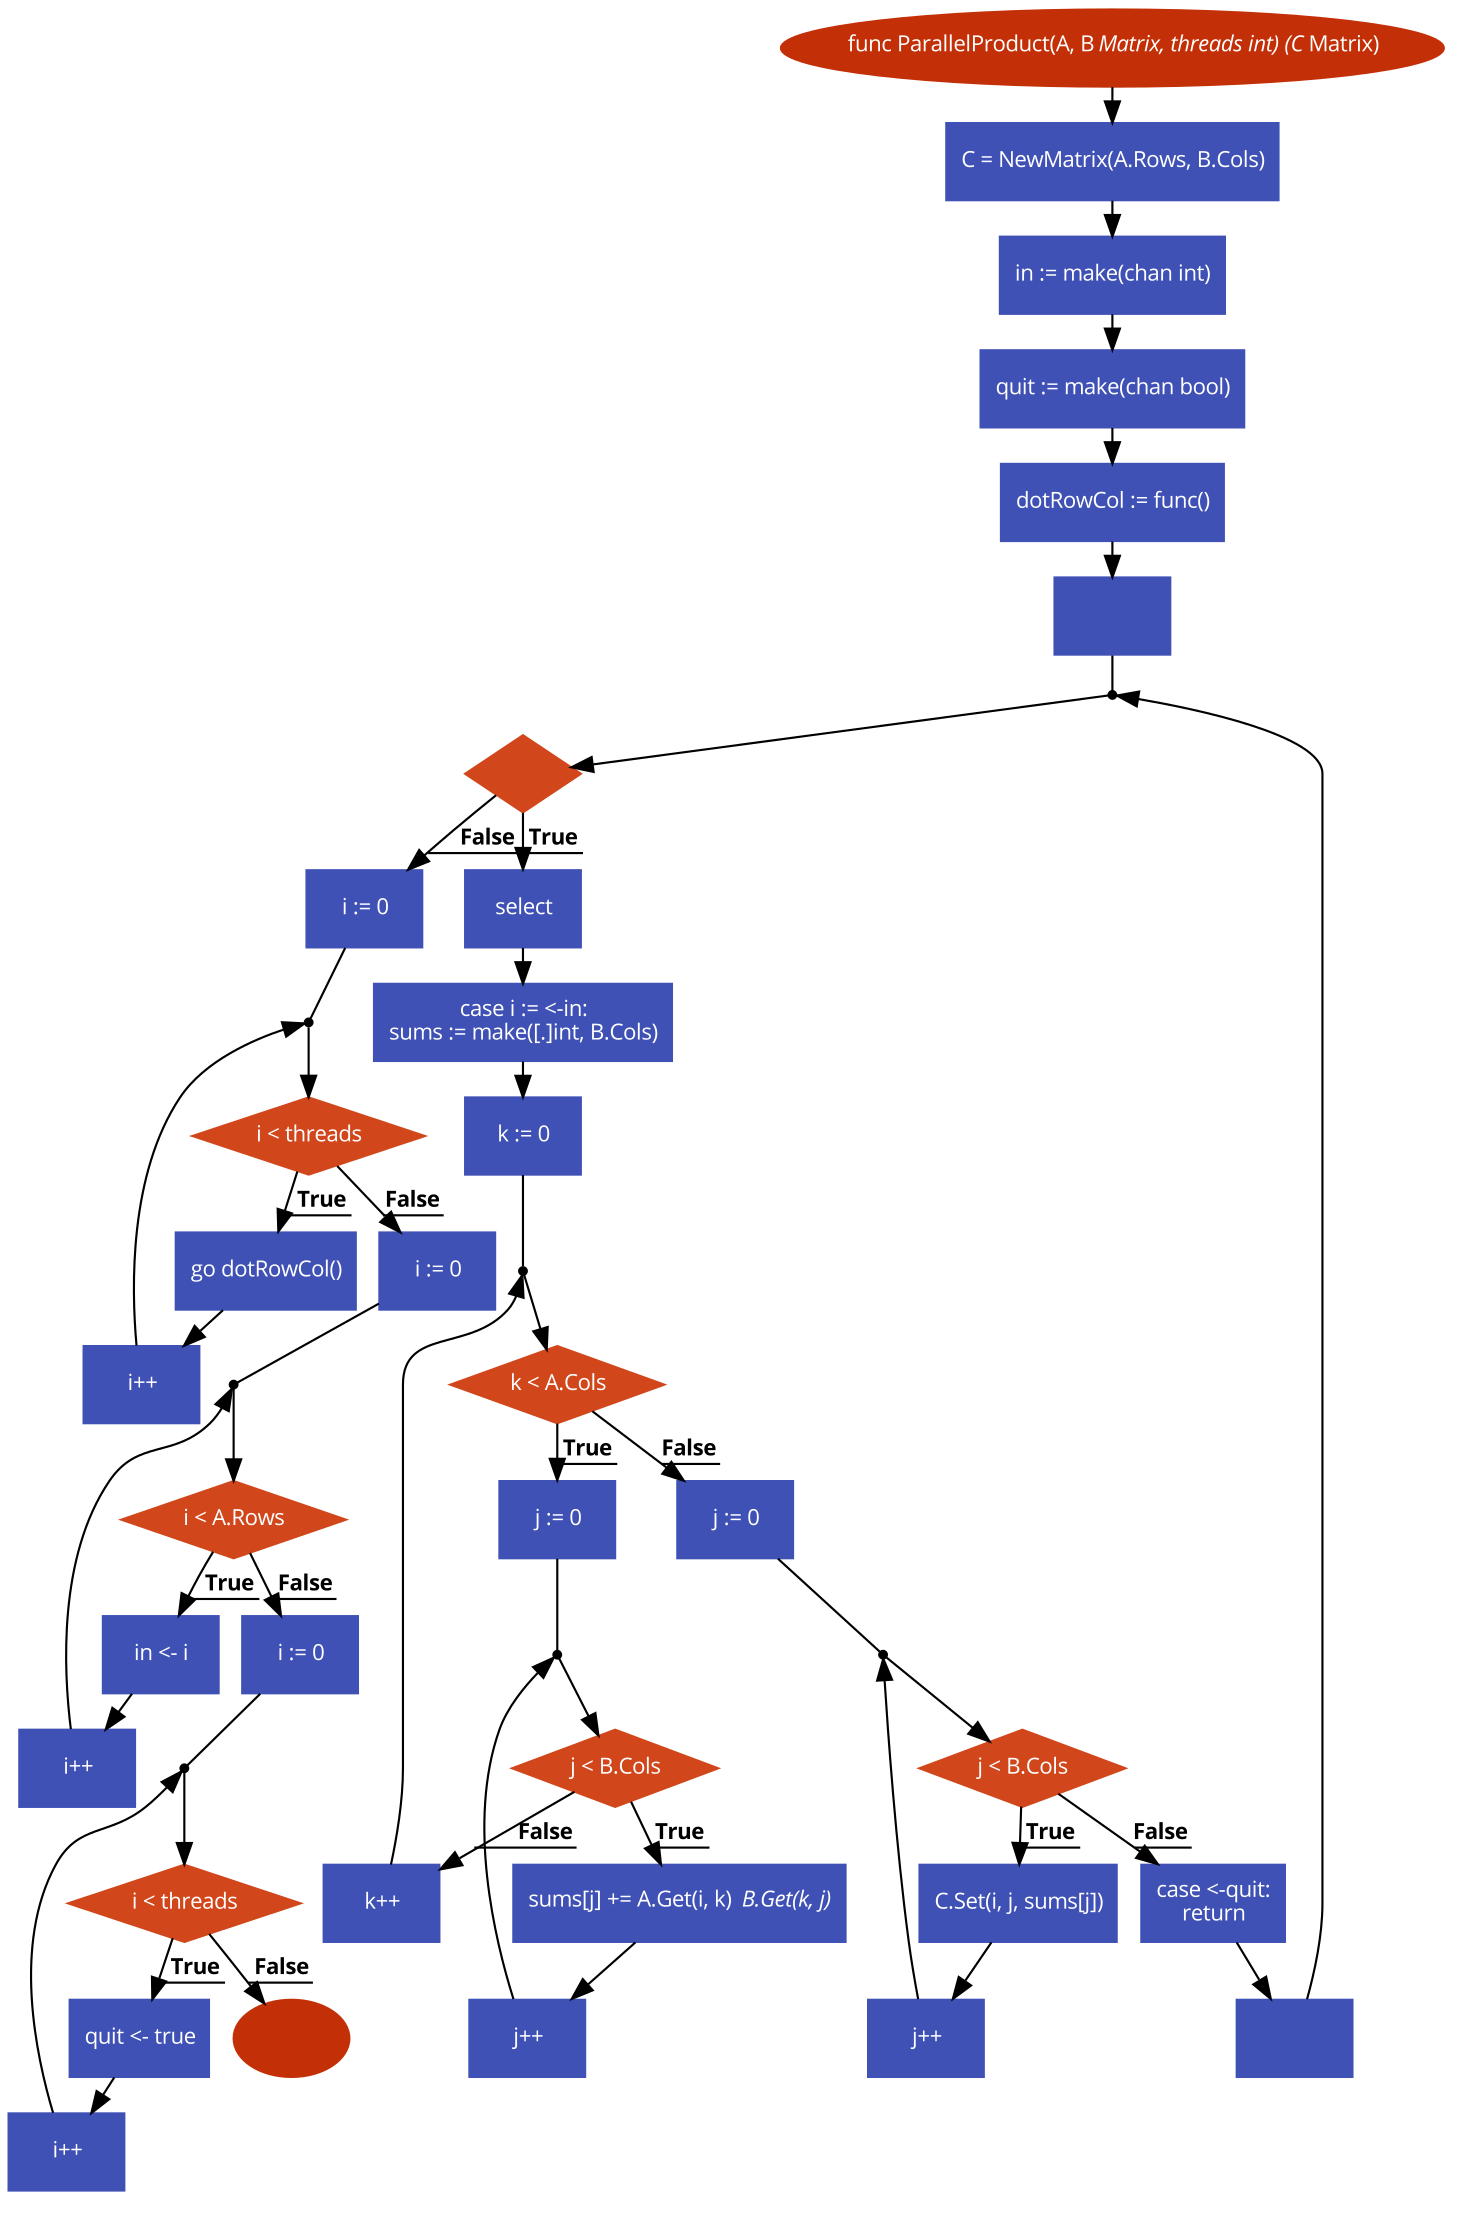
\includegraphics[scale=0.28]{images/matrixParallel.png}
\end{center}

\newpage

\paragraph{Графики}

\begin{flushleft}
	\paragraph{Сравнение работы всех алгоритмов по времени}
\end{flushleft}

\begin{flushleft}
\begin{tikzpicture}
\begin{axis}[
x=0.025cm,
title={Матрицы четных размеров (gobench)},
xlabel={длина строки $l$},
ylabel={время $t(ns)$},
xmin=0, xmax=550,
ymin=0, ymax=3100000000,
xtick={0,50,100,150,200,250,300,350,400,450,500},
ytick={0,500000000,1000000000,1500000000,2000000000,2500000000,3000000000},
legend pos=north west,
ymajorgrids=true,
grid style=dashed,
legend style={at={(0.5,-0.1)},anchor=north},
]

\addplot[
color=red,
mark=square,
]
coordinates {
	(10,18677)(25,279895)(50,2153020)(100,17705457)(200,147803146)(300,660024536)(400,1363797228)(500,3038865567)
};
\addlegendentry{Классический}

\addplot[
color=orange,
mark=square,
]
coordinates {
	(10,11265)(25,157423)(50,1173421)(100,9730347)(200,82138335)(300,335005111)(400,714476506)(500,1548702807)
};
\addlegendentry{Классический с буффером}

\addplot[
color=yellow,
mark=square,
]
coordinates {
	(10,12435)(25,176173)(50,1301969)(100,10412686)(200,88803778)(300,365186425)(400,771183619)(500,1813699928)
};
\addlegendentry{Алгоритм Винограда}

\addplot[
color=green,
mark=square,
]
coordinates {
	(10,12235)(25,163952)(50,1236478)(100,10077546)(200,87102982)(300,367738797)(400,756099434)(500,1656904455)
};
\addlegendentry{Алгоритм Винограда модифицированный}

\addplot[
color=blue,
mark=square,
]
coordinates {
	(10,46465)(25,166977)(50,780152)(100,5364108)(200,41859545)(300,139707371)(400,333703452)(500,645539756)
};
\addlegendentry{Параллельный}

\end{axis}
\end{tikzpicture}
\end{flushleft}

\begin{flushleft}
	\begin{tikzpicture}
	\begin{axis}[
	x=0.025cm,
	title={Матрицы нечетных размеров (gobench)},
	xlabel={длина строки $l$},
	ylabel={время $t(ns)$},
	xmin=0, xmax=550,
	ymin=0, ymax=3100000000,
	xtick={0,50,100,150,200,250,300,350,400,450,500},
	ytick={0,500000000,1000000000,1500000000,2000000000,2500000000,3000000000},
	legend pos=north west,
	ymajorgrids=true,
	grid style=dashed,
	legend style={at={(0.5,-0.1)},anchor=north},
	]
	
	\addplot[
	color=red,
	mark=square,
	]
	coordinates {
		(11,24358)(25,279895)(51,2285599)(101,18134246)(201,144513726)(301,558674691)(401,1409549956)(501,5539562719)
	};
	\addlegendentry{Классический}
	
	\addplot[
	color=orange,
	mark=square,
	]
	coordinates {
		(11,14906)(25,157423)(51,1238208)(101,10047620)(201,78927578)(301,304292664)(401,836216025)(501,3048586554)
	};
	\addlegendentry{Классический с буффером}
	
	\addplot[
	color=yellow,
	mark=square,
	]
	coordinates {
		(11,18015)(25,176173)(51,1506225)(101,10676329)(201,85575794)(301,340706781)(401,900238814)(501,3148107025)
	};
	\addlegendentry{Алгоритм Винограда}
	
	\addplot[
	color=green,
	mark=square,
	]
	coordinates {
		(11,16734)(25,163952)(51,1347086)(101,10253365)(201,82189119)(301,325005796)(401,887266452)(501,3068587535)
	};
	\addlegendentry{Алгоритм Винограда модифицированный}
	
	\addplot[
	color=blue,
	mark=square,
	]
	coordinates {
		(11,48463)(25,166977)(51,794984)(101,5400402)(201,42155935)(301,139336625)(401,343585882)(501,647688412)
	};
	\addlegendentry{Параллельный}
	
	\end{axis}
	\end{tikzpicture}
\end{flushleft}

\newpage

\begin{flushleft}
	\paragraph{Сравнение работы параллельного алгоритма по времени для различного количества горутин}
\end{flushleft}

\begin{flushleft}
	\begin{tikzpicture}
	\begin{axis}[
	x=0.025cm,
	title={Матрицы четных размеров (gobench)},
	xlabel={длина строки $l$},
	ylabel={время $t(ns)$},
	xmin=0, xmax=550,
	ymin=0, ymax=750000000,
	xtick={0,50,100,150,200,250,300,350,400,450,500},
	ytick={0,150000000,300000000,450000000,600000000,750000000},
	legend pos=north west,
	ymajorgrids=true,
	grid style=dashed,
	legend style={at={(0.5,-0.1)},anchor=north},
	]
	
	\addplot[
	color=red,
	mark=square,
	]
	coordinates {
		(10,32020)(25,273434)(50,1513511)(100,10260546)(200,64301722)(300,191698369)(400,385928442)(500,743617280)
	};
	\addlegendentry{Параллельный (2)}
	
	\addplot[
	color=orange,
	mark=square,
	]
	coordinates {
		(10,31746)(25,258196)(50,1176791)(100,5917886)(200,45078104)(300,141235234)(400,333947543)(500,647911588)
	};
	\addlegendentry{Параллельный (4)}
	
	\addplot[
	color=yellow,
	mark=square,
	]
	coordinates {
		(10,24461)(25,188844)(50,793409)(100,5341148)(200,41692136)(300,141491379)(400,330992379)(500,656317703)
	};
	\addlegendentry{Параллельный (8)}
	
	\addplot[
	color=green,
	mark=square,
	]
	coordinates {
		(10,30425)(25,201212)(50,790331)(100,5293963)(200,41345338)(300,146082687)(400,329343441)(500,650544862)
	};
	\addlegendentry{Параллельный (16)}
	
	\addplot[
	color=blue,
	mark=square,
	]
	coordinates {
		(10,46101)(25,167110)(50,800557)(100,5416092)(200,41697141)(300,143526081)(400,329695204)(500,643828218)
	};
	\addlegendentry{Параллельный (32)}
	
	\end{axis}
	\end{tikzpicture}
\end{flushleft}

\begin{flushleft}
	\begin{tikzpicture}
	\begin{axis}[
	x=0.025cm,
	title={Матрицы нечетных размеров (gobench)},
	xlabel={длина строки $l$},
	ylabel={время $t(ns)$},
	xmin=0, xmax=550,
	ymin=0, ymax=750000000,
	xtick={0,50,100,150,200,250,300,350,400,450,500},
	ytick={0,150000000,300000000,450000000,600000000,750000000},
	legend pos=north west,
	ymajorgrids=true,
	grid style=dashed,
	legend style={at={(0.5,-0.1)},anchor=north},
	]
	
	\addplot[
	color=red,
	mark=square,
	]
	coordinates {
		(11,52837)(25,273434)(51,1879390)(101,10895704)(201,59482945)(301,178871008)(401,371193238)(501,753219722)
	};
	\addlegendentry{Параллельный (2)}
	
	\addplot[
	color=orange,
	mark=square,
	]
	coordinates {
		(11,50520)(25,258196)(51,1283508)(101,6019859)(201,42261257)(301,141107153)(401,380434906)(501,666297826)
	};
	\addlegendentry{Параллельный (4)}
	
	\addplot[
	color=yellow,
	mark=square,
	]
	coordinates {
		(11,44191)(25,188844)(51,887298)(101,5471466)(201,42092144)(301,139360513)(401,347229081)(501,649928277)
	};
	\addlegendentry{Параллельный (8)}
	
	\addplot[
	color=green,
	mark=square,
	]
	coordinates {
		(11,43098)(25,201212)(51,844137)(101,5475860)(201,42052141)(301,139242404)(401,339566068)(501,652439038)
	};
	\addlegendentry{Параллельный (16)}
	
	\addplot[
	color=blue,
	mark=square,
	]
	coordinates {
		(11,48463)(25,167110)(51,794984)(101,5400402)(201,42155935)(301,139336625)(401,343585882)(501,647688412)
	};
	\addlegendentry{Параллельный (32)}
	
	\end{axis}
	\end{tikzpicture}
\end{flushleft}

\newpage

\paragraph{Тестовые данные}\\

\begin{flushleft}
	\paragraph{Все алгоритмы}
\end{flushleft}

Время работы в наносекундах для четных размеров матриц (ns):\\
\begin{tabular}{l*{5}{c}r}
	Алгоритм & 10 & 25 & 50 & 100 & 200 \\
	\hline
	Классический & 18677 & 279895 & 2153020 & 17705457 & 147803146 \\
	Классический с буффером & 11265 & 157423 & 1173421 & 9730347 & 82138335 \\
	Алгоритм Винограда & 12435 & 176173 & 1301969 & 10412686 & 88803778 \\
	Алгоритм Винограда модифицированный & 12235 & 163952 & 1236478 & 10077546 & 87102982 \\
	Параллельный & 46465 & 166977 & 780152 & 5364108 & 41859545 \\
\end{tabular}
\begin{tabular}{l*{3}{c}r}
	Алгоритм & 300 & 400 & 500 \\
	\hline
	Классический & 660024536 & 1363797228 & 3038865567 \\
	Классический с буффером & 335005111 & 714476506 & 1548702807 \\
	Алгоритм Винограда & 365186425 & 771183619 & 1813699928 \\
	Алгоритм Винограда модифицированный & 367738797 & 756099434 & 1656904455 \\
	Параллельный & 139707371 & 333703452 & 645539756 \\
\end{tabular}
\\
\\

Время работы в наносекундах для нечетных размеров матриц (ns):\\
\begin{tabular}{l*{5}{c}r}
	Алгоритм & 11 & 25 & 51 & 101 & 201 \\
	\hline
	Классический & 24358 & 279895 & 2285599 & 18134246 & 144513726 \\
	Классический с буффером & 14906 & 157423 & 1238208 & 10047620 & 78927578 \\
	Алгоритм Винограда & 18015 & 176173 & 1506225 & 10676329 & 85575794 \\
	Алгоритм Винограда модифицированный & 16734 & 163952 & 1347086 & 10253365 & 82189119 \\
	Параллельный & 48463 & 166977 & 794984 & 5400402 & 42155935 \\
\end{tabular}
\begin{tabular}{l*{3}{c}r}
	Алгоритм & 301 & 401 & 501 \\
	\hline
	Классический & 558674691 & 1409549956 & 5539562719 \\
	Классический с буффером & 304292664 & 836216025 & 3048586554 \\
	Алгоритм Винограда & 340706781 & 900238814 & 3148107025 \\
	Алгоритм Винограда модифицированный & 325005796 & 887266452 & 3068587535 \\
	Параллельный & 139336625 & 343585882 & 647688412 \\
\end{tabular}

\newpage

\begin{flushleft}
	\paragraph{Параллельные алгоритмы с разным количеством горутин}
\end{flushleft}

Время работы в наносекундах для четных размеров матриц (ns):\\
\begin{tabular}{l*{5}{c}r}
	Алгоритм & 10 & 25 & 50 & 100 & 200 \\
	\hline
	Параллельный (2) & 32020 & 273434 & 1513511 & 10260546 & 64301722 \\
	Параллельный (4) & 31746 & 258196 & 1176791 & 5917886 & 45078104 \\
	Параллельный (8) & 24461 & 188844 & 793409 & 5341148 & 41692136 \\
	Параллельный (16) & 30425 & 201212 & 790331 & 5293963 & 41345338 \\
	Параллельный (32) & 46101 & 167110 & 800557 & 5416092 & 41697141 \\
\end{tabular}
\begin{tabular}{l*{3}{c}r}
	Алгоритм & 300 & 400 & 500 \\
	\hline
	Параллельный (2) & 191698369 & 385928442 & 743617280 \\
	Параллельный (4) & 141235234 & 333947543 & 647911588 \\
	Параллельный (8) & 141491379 & 330992379 & 656317703 \\
	Параллельный (16) & 146082687 & 329343441 & 650544862 \\
	Параллельный (32) & 143526081 & 329695204 & 643828218 \\
\end{tabular}
\\
\\

Время работы в наносекундах для нечетных размеров матриц (ns):\\
\begin{tabular}{l*{5}{c}r}
	Алгоритм & 11 & 25 & 51 & 101 & 201 \\
	\hline
	Параллельный (2) & 52837 & 273434 & 1879390 & 10895704 & 59482945 \\
	Параллельный (4) & 50520 & 258196 & 1283508 & 6019859 & 42261257 \\
	Параллельный (8) & 44191 & 188844 & 887298 & 5471466 & 42092144 \\
	Параллельный (16) & 43098 & 201212 & 844137 & 5475860 & 42052141 \\
	Параллельный (32) & 48463 & 167110 & 794984 & 5400402 & 42155935 \\
\end{tabular}
\begin{tabular}{l*{3}{c}r}
	Алгоритм & 301 & 401 & 501 \\
	\hline
	Параллельный (2) & 178871008 & 371193238 & 753219722 \\
	Параллельный (4) & 141107153 & 380434906 & 666297826 \\
	Параллельный (8) & 139360513 & 347229081 & 649928277 \\
	Параллельный (16) & 139242404 & 339566068 & 652439038 \\
	Параллельный (32) & 139336625 & 343585882 & 647688412 \\
\end{tabular}

\newpage

\paragraph{Оценка трудоемкостей алгоритмов}
\\$A = a\times b$\\$B = b\times c$\\$/ = div$\\$t$ - количество потоков
\begin{itemize}
	\item Классический: $1 + a(3 + c(3 + b(3 + 3 + 7 + 3))) = 1 + 3a + 3ac + 16abc = 1 + 3n + 3n^2 + 16n^3$
	\item Классический с буффером: $1 + a(3 + c(3 + 3 + b(3 + 7) + 3)) = 1 + 3a + 9ac + 10abc = 1 + 3n + 9n^2 + 10n^3$
	\item Алгоритм Винограда: $1 + 1 + a(3 + b/2(3 + 11)) + c(3 + b/2(3 + 11)) + 1 + a(3 + c(3 + 4 + b/2(3 + 18) + 3)) + 2 + \begin{cases} a(3 + c(3 + 3 + 9 + 3)),& \text{if b\%2 != 0}\\0,& \text{otherwise}\end{cases} = 5 + 6a + 3c + 21ab + 10ac + 21bc + 10.5abc + \begin{cases} 3a + 18ac,& \text{if b\%2 != 0}\\0,& \text{otherwise}\end{cases} = 4 + 9n + 54n^2 + 10.5n^3 + \begin{cases} 3n + 18n^2,& \text{if b\%2 != 0}\\0,& \text{otherwise}\end{cases}$
	\item Алгоритм Винограда модифицированный: $1 + 1 + a(3 + b/2(3 + 9)) + c(3 + b/2(3 + 9)) + 1 + 4 + a(3 + c(3 + 4 + b/2(3 + 15) + 1 + \begin{cases} 9,& \text{if b\%2 != 0}\\0,& \text{otherwise}\end{cases} + 3)) = 6 + 6a + 3c + 6ab + 6bc + 9abc + \begin{cases} 20ac,& \text{if b\%2 != 0}\\11ac,& \text{otherwise}\end{cases} + 3bc + 4abc = 6 + 9n + 12n^2 + 9n^3 + \begin{cases} 20n^2,& \text{if b\%2 != 0}\\11n^2,& \text{otherwise}\end{cases}$
	\item Параллельный:
	\begin{enumerate}
		\item $func = 2 + 1 + b(3 + c(3 + 3)) + c(3 + 1) = 3 + 3b + 3c + 6bc = 3 + 6n + 6n^2$
		\item $1 + 1 + 1 + t(3 + func) + a(3 + 1) + t(3 + 2) = 2 + 4a + 8t + func*t = 3 + 4a + 8t + t(3 + 3b + 3c + 6bc) = 3 + 4a + 11t + 3bt + 3ct + 6bct = 3 + 4n + 11t + 3nt + 3nt + 6n^2t$
	\end{enumerate}
\end{itemize}

\newpage

\paragraph{Вывод}

Проделав лабораторную работу были сделаны следующие выводы:
\begin{enumerate}
	\item Из обычных алгоритмов (однопоточных), самым быстрым оказался классический с буффером, а значит улучшения, сделанные в алгоритмах Винограда, на сегодняшний день не имеют особого смысла.
	\item Сравнив обычные алгоритмы с параллельным, было выявлено, что на меньшем количестве элементов, использовать параллельность не имеет особого смысла, он появляется только на больших размерах.
	\item После сравнения параллельного алгоритма с разным количеством горутин, можно утверждать, что количество горутин, которые могут одновременно жить в системе для оптимальной работы алгоритма $\geq 2*n \leq 16*n$, где $n$ - количество реальных ядер процессора. Менее не имеет смысла и более тоже, исходя из графиков. 
\end{enumerate}
Подводя итог, можно сказать, что самым оптимальным способом перемножения матриц будет являться общий алгоритм, где если $n$ - небольшое число, то использовать классический алгоритм с буффером, иначе параллельный.

\paragraph{Заключение}

В ходе работы были описаны и реализованы различные варианты алгоритма перемножения матриц (классический, классический с буффером, алгоритм Винограда, модифицированный алгоритм Винограда и параллельный), и был проведен сравнительный анализ их временной эффективности.

\backmatter %% Здесь заканчивается нумерованная часть документа и начинаются ссылки и
            %% заключение

\appendix   % Тут идут приложения

\end{document}

%%% Local Variables:
%%% mode: latex
%%% TeX-master: t
%%% End: